%%% Document Author: J Moss
%%% Parts in LaTeX: Nicholas Dart
%%% Other Content: See authors list
%%% Document Last edit: 28.10.2014

\documentclass[11pt, titlepage]{article}
\usepackage{a4wide}
\usepackage[english]{babel}
\usepackage{graphicx}
\usepackage{tabu}
\usepackage{textcomp}
\usepackage{fancyhdr}
\usepackage{lastpage}
\usepackage{titlesec}

\title{ \huge CS221 Group Project \\ \Large Project Plan}
\author{
	\vspace{100pt}
	\begin{tabular}{ r || l }
		Project Team 	& jcm14, acb12, mta12, wia3, \\
						& nid21, msh4, jao14, mip34, \\
	 					& set12, daw54, anw46 \\
						& \\
		Version			& 0.4 \\
		Status			& Pre-Release \\
		Date Published  & \today \\
		Reference 		& SE\_NO2\_MAN\_01 \\
		Department		& Computer Science \\
		Address			& Aberystwyth University \\
						& Penglais Campas \\
						& Ceredigion \\
						& SY23 3DB \\
	\end{tabular} \\
	Copyright \textcopyright Aberystwyth University 2014
}

\pagestyle{fancy}
\fancyhf{}
\rfoot{Page \thepage \hspace{1pt} of \pageref{LastPage}}
\lfoot{Aberystwyth University - Computer Science}

\begin{document}
	\setcounter{page}{1}
	\maketitle
	\clearpage
	\tableofcontents
	\newcommand{\sectionbreak}{\clearpage} 	%% Allways start a section on a new page
	\clearpage
	\section{Introduction}
		\subsection{Purpose of this Document}
			This document has been commissioned to show our current understanding of the client's requirement specification of Reserve Plant Species Recording ("RPSR"). The project encompassing the Android Application Framework and modern Web Technologies which will provide a monitoring system for definable Areas of Interest, into a series of basic objectives and milestones. RPSR has three main component parts, an Android Application, a Website and a Database.
			
			The document will give a high level overview of the time line for developing and testing RPSR, an estimate of the final User Interface design, a probabilistic risk assessment, and a use case breakdown.

			The client is to read this document and confirm that their requirements have been understood and correctly interpreted by the team.
		\subsection{Scope}
			The document comprises the high level design and development plan for RPSR, it should not be referred to for final software design structure. This document will follow the design specification.
			
			This document provides an overview of the system we have interpreted for the client, including our choice of platform (where applicable), high-level architecture and will also included a section dedicated out understanding of the target audience of the application.
			
			A use case diagram and corresponding table will show how the actors of the system are expected to interact with elements of the system. The document will also contain a probabilistic risk assessment for the project in full.
			This document will provide a first draft of the UI designs and are subject to alterations at a later date.\\
		\subsection{Objectives}
			The objective of this document is to show our initial plan for development of RPSR, from initial UI designs and user interaction plans, through a breakdown of deliverable dates on a Gantt chart and the expected issues that could arise during development. This is as follows:
			\begin{enumerate}
			\item Provide a high level overview of system design and interaction
			\item Define the technologies used for the system
			\item Display the initial web UI
			\item Display the initial Android UI
			\item Breakdown the project into milestones
			\item Define a limited scope risk assessment for the project and the plans to mitigate the risks
			\end{enumerate}
	\section{Overview}
		\subsection{Platforms}
			\subsubsection{Android}
				The client placed a specific request for the application to run on Android devices. As yet no response has been received for a minimum version, so keeping with more up to date releases, we will use Android API 15 (Android 4.0.3 which encompasses the vast majority of new Smart Phones)
			\subsubsection{LAMP Server}
				We will be using a LAMP Server; Linux, Apache2, MySQL, and PHP ready server. This will provide us with the tools ready to develop the website, and interact with the database.
				PHP was chosen to handle the server side processing of received data due to it's free and wide availability. The language is also covered in other modules during the project time line, meaning it will be fresh in the minds of the web team.
				MySQL is the most commonly used database software on web servers.
		\clearpage
		\subsection{High Level Architecture}
		The system consists of the following high-level elements:
			\subsubsection{Android Application (RPSRrec)}
		
			The application fulfils the following roles:
			\begin{itemize} \itemsep0pt
				\item Collect information about a new visit from the user
				\item Allow the user to record a new visit each time they complete one
				\item Collect time and date data from the phone for the recordings
				\item Allow the user to select a species to use from the database
				\item Take a photo using the Android device by capturing a new photo or selecting
                    from the device's library
				\item Allow the user to enter data for each species
				\begin{itemize}
					\item Typical location
					\item Abundance using "DAFOR" scale
					\item Free text comment
					\item Photo of the general scene at the typical location
					\item Photo of the specimen
					\item Allow the user to enter a name of a new species if not currently available
				\end{itemize}
				\item Allow the user to edit and delete local (not yet uploaded) recordings
		    		and the species data within them.
				\item Obtain location data from the GPS unit within the mobile device to include
				    in the recording
				\item Upload the collected recordings to the remote database server whenever 
		    		a network connection becomes available
		    \end{itemize}
        \clearpage
        \subsubsection{Website (RPSRview)}
            
            The website fulfils the following roles:
            
            	\begin{itemize} \itemsep0pt
            		\item Browse and search uploaded recordings
                	\item Provide detailed view of individual recordings
                	\item Enable maintenance of recordings database
                \end{itemize}
                
        \subsubsection{Server (RPSRsrv)}
        
            The server fulfils the following roles:
            \begin{itemize} \itemsep0pt
                \item Provide a public Web API to be used by the website and the mobile application,
                      enabling safe HTTP access to stored recordings
                \item Provide a MySQL database for the Web API to use as a data store
                \item Ensure data integrity and security
			\end{itemize}
		\subsection{Target Audience}
			The client stated:\\ \\ \indent \textit{The system will be used by naturalists who are familiar with standard computer interfaces. They are concerned 
with accuracy of recording and they may have to operate in difficult weather conditions and in remote locations.}\\ \\
From this we understood the users will be competent in the basic interaction with Android and Web User Interfaces. We have designed the application to have large areas for input to aid in quick input when outdoors and reduce unused space on a minimal screen real estate. We have designed the application to work in the first case without Internet connectivity, and when it becomes available, then offer to upload the work produced offline.


	\section{Use Cases}
		\subsection{Use Case Diagram}
			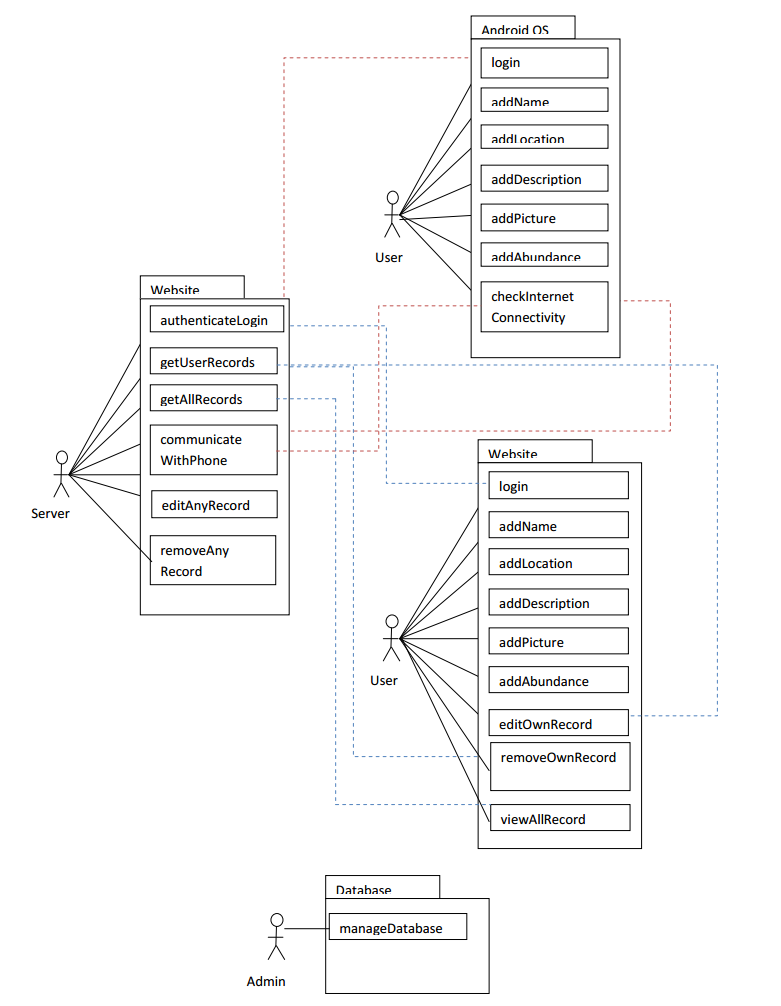
\includegraphics[scale=0.8]{res/UseCaseDiagram.png}
		\subsection{Use Case Descriptions}
		
			\begin{tabu} to 1\textwidth {X[l] | X[l]}
			
				\hline \textbf{Android OS User} & \\ \hline \\
				Login & User should be able to log into the application by entering a valid username and/ or password \\
					addName & user should be able to add the name of a plant to the database \\
					addLocation & user should be able to add the location of a plant to the database \\
					addDescription & user should be able to add a description of the plant to the database \\
					addPicture & user should be able to add a picture of the plant to the database \\
					addAbundance & user should be able to record the level of abundance of the plant within the area \\
					checkInternetConnectivity & the application should be able to know if it is connected to the internet and is able to send records to the database. If not the data is stored in local storage \\
				\hline \textbf{Website User} &  \\ \hline \\
					Login & User should be able to log into the application by entering a valid username and/ or password \\
					addName & user should be able to add the name of a plant to the database \\
					addLocation & user should be able to add the location of a plant to the database \\
					addDescription & user should be able to add a description of the plant to the database \\
					addPicture & user should be able to add a picture of the plant to the database \\
					addAbundance & user should be able to record the level of abundance of the plant within the area \\
					editOwnRecord & user should be able to make changes to any record that they have added to the database \\
					removeOwnRecord & user should be able to remove any record that they have added to the database \\
					viewAllRecord & user should be able to view any record in the database through the website \\
				\end{tabu}
				\clearpage
				\begin{tabu} to 1\textwidth {X[l] | X[l]}
				\hline \textbf{Administrator} &  \\ \hline \\
					manageDatabase & the administer must be able to access the database and manage / maintain the database \\
				\hline \textbf{Server} &  \\ \hline \\
					authenticateLogin & the server will allow a user to log onto the application through their phone or through the website providing that the user has entered correct username and/or password \\
					getUserRecords & when the user wants to view edit or delete records they have entered the server will need to call them from the database \\
					getAllRecords & the server will send information about all the records in the database to the user upon request \\
					communicateWithPhone & server must be able to send and receive data from the phone of records being entered \\
					editAnyRecord & the website admin should be able to edit any record entered in the database by any user \\
					removeAnyRecord & the website admin should be able to remove any record entered into the database by any user \\
				\end{tabu}
		\clearpage
	\section{User Interface Designs}
		\subsection{Android Interface}
			This section displays the envisioned design of the Android Application layout.
			\subsubsection{New Site Visit}
			\begin{center}
			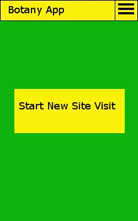
\includegraphics[scale=1]{res/botanyAppNewSiteVisit1.png}
			 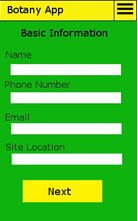
\includegraphics[scale=1]{res/botanyAppNewSiteVisit2.png}
			\end{center}
			
			The first thing that will be presented to the user on entry to the app will be the option to create a new visit by pushing the button provided. This will then load the Basic Information page.\\

			The user will then be prompted to input their basic information such as their name, phone number, email and site location for reference. These are to be validated by the server upon the push of the Next button. 					Add a species page will then be displayed to the user.\\
			
			Further fields may be required to be added at a later date due to additional requirements given by the client or by a change during further 																						development in the design.\\
			
			There is no requirement in the spec to remember the user’s details on the app so currently the user will have to fill in their details each time 																					they make a recording.\\
				
			\subsubsection{Adding a new species}
			\begin{center}
			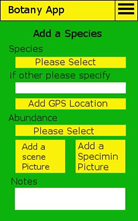
\includegraphics[scale=1]{res/botanyAppAddSpecies1.png}
			 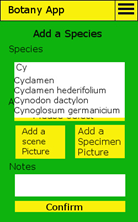
\includegraphics[scale=1]{res/botanyAppAddSpecies2.png}
			\end{center}
			The first input asked of the user is to select a species to record using an integrated search function. This will not only help the user find the species they are looking for, but also allow the user to add a new species to the database if required.\\
			
			An option to provide a GPS signal is given which will link up with the GPS in the android device to provide a location. Options are given to provide pictures of the site and specimen either from the camera or the gallery on the device. A field for adding notes will be provided that may be useful to the record.\\
			\clearpage
			\subsubsection{Editing and saving a site visit}
						\begin{center}
			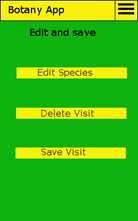
\includegraphics[scale=1]{res/botanyAppEditSaveSiteVisit.png}
			\end{center}
			The edit and save page provides the options to the user to view and edit the recordings made. The Edit Species link allows the user to access a list of the species pages they have added to the visit. This takes the user back to the Add a Species page to edit or delete an entry.\\
			
Users are given the option to delete the visit which will be met with a prompt to confirm or cancel the delete.\\

 The final link is to save all recordings, giving permission to upload the data to the database at an appropriate time.\\
\clearpage
				
		\subsection{Web Interface}
		This section displays the envisioned design of the Website Layout
		
		\subsubsection{Web Homepage}
			\begin{center}
				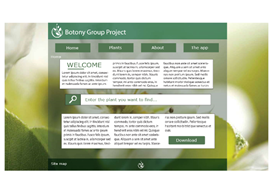
\includegraphics[scale=1]{res/botanyWebHome.png}
			\end{center}
			The Homepage has a central search bar to search the database for visit records and species information. The navigation bar at the top remains consistent over all pages with breadcrumbs just below to ensure ease of navigation. There is a link to the site map in the footer which also remains consistent.
There will be a heading welcoming the user, alongside information regarding the nature and purpose of the website. 

		\subsubsection{Plant Database Page}
			\begin{center}
				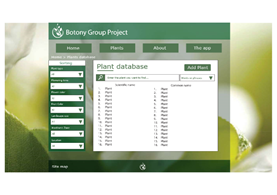
\includegraphics[scale=1]{res/botanyWebPlantDatabase.png}
			\end{center}
			The plant database provides access to the entire database using the search bar to search plants by name. The search results will be displayed as a list. 
At the side there is a sorting bar which contains various drop down menus of search filters to refine the search if required. The user can then click a record which will be linked to the plants details (4.7).
The Add Plant button will link the user to the Add record page.

		\subsubsection{Add Record Page}
			\begin{center}
				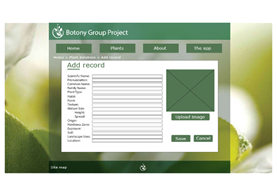
\includegraphics[scale=1]{res/botanyWebAddRecord.png}
			\end{center}
			This page allows the user to add a new record to the database. The user will be asked to provide information such as scientific name, pronunciation, common name, origin and location alongside an image that can be uploaded to the database upon clicking the save button. 
		\subsubsection{Plant Details Overlay}
			\begin{center}
				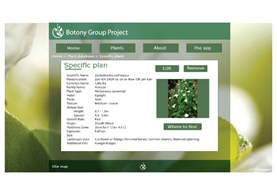
\includegraphics[scale=1]{res/botanyWebPlantDetailsOverlay.png}
			\end{center}
			The specific plant page allows the user to access data about individual plants. Above the picture there are links to edit and remove the records giving the user the ability to update the data about the plant. A where to find button links to a map of the location based from GPS coordinates.
					\subsubsection{Plant Location Overlay}
			\begin{center}
				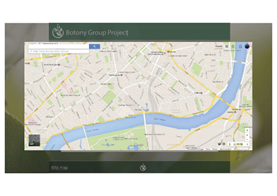
\includegraphics[scale=1]{res/botanyWebPlantMap.png}
			\end{center}
			Upon clicking the Where to Find button, a map will open displaying the location of the selected plant using the location from the database.
Note: Use of Google Maps.
			\subsubsection{Remove Plant Record}
			\begin{center}
				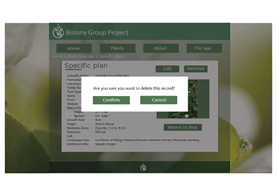
\includegraphics[scale=1]{res/botanyWebPlantRemoval.png}
			\end{center}
			If the user chooses to remove a record they can do so by pressing the Remove button where they will be prompted to verify their choice before the entry is deleted.
			
			\clearpage
	\section{Gantt Chart}
		Note: This was difficult to format properly so is included as a web link until a clear format without loss of emphasis can be applied.
		
	\section{Risk Analysis and Mitigation}
	\begin{tabular}[]{| p{3cm} | c | c | c | p{5cm} |}
\hline
\textbf{Ongoing}&\textbf{Likelyhood}&\textbf{Magnitude}&\textbf{Risk}&\textbf{Mitigation} \\ \hline \hline%\hhline{|=|=|=|=|=|}
Planned Team Member Absence &2&2&4&Meetings scheduled in advance with plenty of time for members to state if there is a problem attending. Missing member required to read minutes and report to relevant manager. \\ \hline
Planned Project Leader Absence&2&3&6&Meeting to be chaired by Deputy Project Leader instead. \\ \hline
Planned QA Manager Absence&2&3&6&QA Questions and Decisions to be made by Deputy QA Manager instead. \\ \hline
Unplanned Team Member Absence &3&2&6&Missing member reqired to read minutes and reprot to manager. Persistant lack of attendence to result in being carded. \\ \hline
Unplanned Project Leader Absence&3&3&9&"Persistant lack of attendence to result in Deputy taking over\\ \hline
Unplanned QA Manager Absence&3&3&9&"Persistant lack of attendence to result in Deputy taking over\\ \hline
Github Downtime&1&2&2&Local copies to be used. \\ \hline
Github Failure&1&3&3&Use backup to host locally. \\ \hline
Long term illness&1&3&3&"Member to report to relevant manager in advance\\ \hline
Member dropout&1&4&4&"Member to report to relevant manager in advance\\ \hline
\end{tabular}

\begin{tabular}[]{| p{3cm} | c | c | c | p{5cm} |}
\hline
\textbf{Documentation}&\textbf{Likelyhood}&\textbf{Magnitude}&\textbf{Risk}&\textbf{Mitigation} \\ \hline \hline

Individual parts of document submitted late&2&3&6&Internal Deadline set as Friday before the tutorial meeting. Team Members to report to relevant manager as soon as an issue with making the deadline is apparent. \\ \hline
Individual parts of document submitted with low quality&2&3&6&"Documents to be read by entire team\\ \hline
Human Errors&3&2&6&"Documents should be reviewed by relevent managers and the QA manager\\ \hline
\end{tabular}

\begin{tabular}[]{| p{3cm} | c | c | c | p{5cm} |}
\hline
\textbf{Software Development and Delivery}&\textbf{Likelyhood}&\textbf{Magnitude}&\textbf{Risk}&\textbf{Mitigation} \\ \hline \hline
Slipping from Project Timeline&2&3&6&"Detailed gant charts and time predictions should be kept and viewable by all\\ \hline
Missing or incomplete parts of implementation&2&4&8&Project Leader to make sure tasks exist for all objectives. QA Manager to ensure work is progressing satisfactory. Extensive testing to make sure all features work as expected. \\ \hline
Feature Creep&2&2&4&Teams to maintain communcation with managers. QA Manager to maintain adherence to objectives. \\ \hline
Implementation not working as expected by client&2&3&6&Project Leader to practice strong expectation management. \\ \hline
Client requirements change&2&2&4&"Keep regular contact with the client\\ \hline

\end{tabular}
\clearpage
	\section{References}
		Not Applicable

	\section{Document History}
		\begin{tabular}{l || c | l}
		Version Number & Edit & Date \\ \hline 
		& & \\
		0.1 & Initial Version & October 21 2014 \\
		0.2 & Document First Draft & October 27 2014 \\
		0.3 & Client first release & October 28 2014 \\
		0.4 & Spellchecking and Document standardization & October 29 2014 \\
		
		\end{tabular}
\end{document}